% Author = dyfmeks
% Date = 20/05/2024

% Preamble
\documentclass[stu, 12pt, letterpaper, donotrepeattitle, floatsintext, natbib]{apa7}
\setlength{\headheight}{15.35403pt}

% Packages
\usepackage[utf8]{inputenc}
\usepackage{comment}
\usepackage{marvosym}
\usepackage{graphicx}
\usepackage{float}
\usepackage[normalem]{ulem}
\usepackage[spanish]{babel}
\usepackage{apacite}
\usepackage{tabularx}
% \usepackage[style=apa,sortcites=true,sorting=nyt,backend=biber]{biblatex}
\usepackage{standalone}
\usepackage{csquotes}
\selectlanguage{spanish}
\useunder{\uline}{\ul}{}
\newcommand{\myparagraph}[1]{\paragraph{#1}\mbox{}\\}
%\usepackage[section]{placeins}
%\usepackage{csquotes}
%\usepackage{array,fancyvrb,graphicx,verbatim,xurl}

% Config
%\DeclareLanguageMapping{american}{american-apa}
%\addbibresource{bibliography.bib}
\thispagestyle{empty}
\title{\large OPTIMIZACI\'ON DE LA GESTI\'ON DE INVENTARIO DE EQUIPOS MEDIANTE EL DISE\~{N}O E IMPLEMENTACI\'ON DE UN MODULO CON GESTI\'ON DE MOVIMIENTOS Y REPORTES}
\shorttitle{Gesti\'on de Inventario de Equipos}
\author{John Jordan Quispe Supo}
\authorsaffiliations{Instituto de Educaci\'on Superior Privado del Sur}
\course{Desarrollo de Sistemas de Informaci\'on}
\professor{Gustavo Delgado Ugarte}
\duedate{20/05/2024}

%\abstract{Este proyecto se centra en el dise\~{n}o y desarrollo de un Sistema de Informaci\'on Integral para la Gesti\'on de
%Conquistadores, Actividades y Progresos en el Club de Conquistadores. El sistema propuesto permitir\'a el registro de
%nuevos conquistadores, la planificaci\'on y registro de actividades, el seguimiento del avance de los conquistadores en
%sus especialidades y clases, y la toma de asistencia y actividades semanales en la unidad. Este trabajo busca optimizar
%la gesti\'on del club, mejorar la eficiencia de las actividades y proporcionar una plataforma web para el seguimiento y
%desarrollo de los conquistadores. Se espera que este sistema integral mejore significativamente la administraci\'on del
%club y enriquezca la experciencia de los conquistadores.}
%\keywords{Sistema de Informaci\'on Integral, Gesti\'on de Conquistadores, Registro de Actividades, Seguimiento de Progresos,
%Club de Conquistadores, Planificaci\'on de Actividades, Toma de Asistencia, Actividades Semanales, Especialidades y Clases
%de Conquistadores, Plataforma Web, Optimizaci\'on de la Gesti\'on, Eficiencia de las Actividades}

% Document
\begin{document}
\maketitle

%   Indices
\pagenumbering{roman}
%   Contenido
\renewcommand\contentsname{\large\'Indice}
\tableofcontents
\setcounter{tocdepth}{2}
\newpage
%   Figuras
\renewcommand\listfigurename{\large\'Indice de figuras}
\listoffigures
\newpage
%   Tablas
\renewcommand\listtablename{\large\'Indice de tablas}
\listoftables
\newpage

%   Cuerpo
\pagenumbering{arabic}

% \section{\large T\'ITULO}
% \noindent OPTIMIZACI\'ON DE LA GESTI\'ON DE INVENTARIO DE EQUIPOS MEDIANTE EL DISE\~{N}O E IMPLEMENTACI\'ON DE UN MODULO CON GESTI\'ON DE MOVIMIENTOS Y REPORTES

% \section{\large DATOS DEL AUTOR}
% \begin{tabular}{@{} p{2cm} p{12.8cm} @{}}
%     \textbf{Nombres}   & : John Jordan                                                                                            \\
%     \textbf{Apellidos} & : Quispe Supo                                                                                            \\
%     \textbf{Carrera}   & : Desarrollo de Sistemas de Informaci\'on                                                                \\
%     \textbf{Rese\~{n}a}    & : Soy egresado del Instituto del Sur y actualmente laboro en Soluciones de Informaci\'on NextSoft S.A.C. \\
% \end{tabular}
% \newline

% \section{\large RESUMEN}
% El presente proyecto se centra en el desarrollo de un m\'odulo de gesti\'on de inventario de equipos, dise\~{n}ado para optimizar el control de recursos en una organizaci\'on. Este m\'odulo permite el registro
% detallado de equipos, la gesti\'on de movimientos (entregas a responsables, devoluciones a almac\'en) y las transferencias entre almacenes. Adem\'as, incluye funcionalidades para el mantenimiento de datos
% maestros como marcas, modelos, productos y categor\'{\i}as. El sistema tambi\'en genera reportes exhaustivos que facilitan la toma de decisiones, mejorando la eficiencia en la administraci\'on de los equipos.
% La implementaci\'on del m\'odulo fue realizada utilizando tecnolog\'{\i}as actuales, asegurando su integrabilidad y escalabilidad dentro de la infraestructura existente de la organizaci\'on.


\section{\large Introducci\'on}
\subsection{Contexto y Antecedentes}
\subsubsection{Descripci\'on de la Unidad de Estudio}
% \begin{tabular}{@{} p{4.3cm} p{9.5cm} @{}}
%     \textbf{RUC}                   & : 20454819137                                                                                                                                         \\
%     \textbf{Raz\'on Social}        & : Soluciones de Informaci\'on NextSoft S.A.C.                                                                                                         \\
%     \textbf{Inicio de Actividades} & : 01/05/2008                                                                                                                                          \\
%     \textbf{Actividad principal}   & : Brinda soluciones informáticas a través de un sistema ERP personalizado y desarrollos a medida para empresas locales, nacionales e internacionales.
% \end{tabular}
El presente proyecto se llevar\'a a cabo en Soluciones de Informaci\'on NextSoft S.A.C. con RUC 20454819137, una empresa especializada en el desarrollo de soluciones tecnol\'ogicas para la gesti\'on empresarial.
Fundada con el objetivo de ofrecer productos y servicios de alta calidad en el \'ambito de la tecnolog\'{\i}a de la informaci\'on, NextSoft S.A.C. se ha consolidado como un actor relevante en el sector, destac\'andose
por su innovaci\'on y compromiso con la satisfacci\'on del cliente.

\textbf{Misi\'on. }Brindar a nuestros clientes, soluciones de negocio de la m\'as alta calidad, utilizando tecnolog\'{\i}as innovadoras y pertinentes que permitan el aumento de la productividad.

\textbf{Visi\'on. }Constituirnos en un elemento fundamental de apoyo a nuestros clientes llegando a convertirnos en la empresa líder del medio, al entregar soluciones innovadoras que satisfagan a nuestros clientes quienes
son nuestra raz\'on de ser.

\textbf{Estructura Organizativa. }NextSoft S.A.C. cuenta con un equipo multidisciplinario de profesionales altamente capacitados en diversas \'areas de la tecnolog\'{\i}a de la informaci\'on. La empresa se organiza en
departamentos clave, como desarrollo de software, soporte t\'ecnico y atención al cliente, todos ellos coordinados para ofrecer un servicio integral y de alta calidad.

\textbf{Relevancia en el Sector. }Gracias a su enfoque en la innovaci\'on y la calidad, NextSoft S.A.C. ha logrado posicionarse como un proveedor confiable de soluciones tecnol\'ogicas para diversas industrias. Su capacidad
para adaptarse a las necesidades cambiantes del mercado y ofrecer productos personalizados ha sido fundamental para su crecimiento y reconocimiento en el sector.

\subsubsection{Diagn\'ostico de la Situaci\'on Actual}
En la actualidad, la gesti\'on de inventario de equipos en diversas empresas presenta desaf\'{\i}os significativos, debido a la falta de herramientas espec\'{\i}ficas que permitan un control eficiente y centralizado. Muchas
organizaciones dependen de sistemas manuales o soluciones tecnol\'ogicas gen\'ericas que no est\'an adaptadas a las necesidades particulares de la gesti\'on de equipos. Esto resulta en procesos ineficaces, errores en el
registro de datos, dificultades en el seguimiento de movimientos y transferencias de equipos, y una visibilidad limitada sobre el estado y la ubicaci\'on de los recursos.

\textbf{Sistemas y Procesos Existentes. }En la mayor\'{\i}a de las empresas, la gesti\'on de inventarios de equipos se lleva a cabo mediante hojas de c\'alculo o software b\'asico de gesti\'on, que no est\'an dise\~{n}ados
espec\'{\i}ficamente para manejar la complejidad de los movimientos, entregas, devoluciones y transferencias de equipos entre almacenes. Estos m\'etodos suelen ser propensos a errores humanos, carecen de funcionalidades
avanzadas para la generaci\'on de reportes detallados y no permiten un seguimiento en tiempo real, lo que complica la toma de decisiones informadas.

\textbf{Deficiencias y \'Areas de Mejora. }Entre las principales deficiencias de los sistemas actuales se encuentra la falta de integrabilidad con otros sistemas de la empresa, la ausencia de control de estados para el
mantenimiento de equipos o el seguimiento de su ciclo de vida, y la incapacidad para generar reportes que ofrezcan una visi\'on clara y actualizada del estado del inventario. Adem\'as, la falta de un sistema centralizado
para la gesti\'on de marcas, modelos y categor\'{\i}as de equipos dificulta el an\'alisis y la planificaci\'on de compras o reposiciones.

\textbf{Oportunidad de Mejora. }La implementaci\'on de un m\'odulo espec\'{\i}fico para la gesti\'on de inventario de equipos, que contemple no solo el registro y control de los equipos, sino tambi\'en la gesti\'on de
movimientos, transferencias entre almacenes, y la generaci\'on de reportes, representa una oportunidad significativa para optimizar estos procesos. Este m\'odulo est\'a dise\~{n}ado para ser adaptable y escalable, permitiendo
su implementaci\'on en diferentes empresas que requieran mejorar su gesti\'on de inventarios, independientemente de su tama\~{n}o o sector.

La soluci\'on propuesta busca atender estas deficiencias, proporcionando a las empresas una herramienta robusta y especializada que facilite la gesti\'on integral de sus inventarios de equipos, mejorando la eficiencia
operativa y la precisi\'on en el manejo de recursos.
\subsection{Problema de Investigaci\'on}

\subsubsection{Definici\'on del Problema}
Este proyecto aborda la necesidad de un sistema de informaci\'on integral que
optimice la gesti\'on de los miembros, las actividades y el seguimiento de los
progresos dentro de un Club de Conquistadores. Actualmente, la administraci\'on
de estos elementos se realiza de manera manual o con herramientas dispersas, lo
que conlleva a ineficiencias y dificultades en el seguimiento y evaluaci\'on
del desarrollo de los conquistadores. Por tanto, se propone el dise\~{n}o y
desarrollo de una soluci\'on inform\'atica que centralice la informaci\'on y
automatice los procesos, mejorando as\'i la gesti\'on y el impacto de las
actividades del club.

\subsection{Objetivo General}
Desarrollar un sistema de informaci\'on integral que facilite la gesti\'on
eficiente de los miembros, actividades y progresos del Club de Conquistadores,
proporcionando una herramienta tecnol\'ogica que optimice los procesos
administrativos y de seguimiento, garantizando la mejora continua en la
organizaci\'on y participaci\'on de los conquistadores.

\subsection{Objetivos Espec\'ificos}
\begin{enumerate}
    \item\textbf{Automatizar el registro y gesti\'on de conquistadores:}\\Implementar funcionalidades que permitan el registro detallado de nuevos conquistadores, incluyendo sus datos personales, informaci\'on de contacto y estado de inscripci\'on, asegurando un manejo eficiente y seguro de la informaci\'on.
    \item\textbf{Registrar y monitorear actividades del club:}\\Dise\~{n}ar y desarrollar m\'odulos que permitan la planificaci\'on, organizaci\'on y seguimiento de las actividades y eventos del club, facilitando la coordinaci\'on y participaci\'on activa de los miembros.
    \item\textbf{Controlar el progreso de especialidades y clases:}\\Implementar un sistema de seguimiento individualizado para registrar y monitorear el avance de los conquistadores en sus especialidades y clases, proporcionando informes detallados y estad\'isticas de progreso.
    \item\textbf{Gestionar la asistencia a actividades y reuniones:}\\Crear un m\'odulo para el registro y control de asistencia de los conquistadores en las actividades semanales y eventos especiales, facilitando la evaluaci\'on de la participaci\'on y compromiso de los miembros.
    \item\textbf{Desarrollar un portal de usuario:}\\Dise\~{n}ar una interfaz amigable y accesible para que los conquistadores y sus l\'ideres puedan consultar y actualizar informaci\'on relevante, facilitando la comunicaci\'on y el acceso a recursos y materiales del club.
    \item\textbf{Generar informes y estad\'isticas:}\\Implementar herramientas de generaci\'on de informes y estad\'isticas que permitan a los l\'ideres del club evaluar el desempe\~{n}o y progreso de los conquistadores, as\'i como la efectividad de las actividades realizadas.
    \item\textbf{Garantizar la seguridad y confidencialidad de la informaci\'on:}\\Establecer mecanismos de seguridad que aseguren la protecci\'on de los datos personales y la confidencialidad de la informaci\'on gestionada por el sistema, cumpliendo con las normativas legales vigentes.
\end{enumerate}

\section{Marco Te\'orico}

\subsection{Introducci\'on al Club de Conquistadores}
El Club de Conquistadores es una organizaci\'on juvenil que promueve el
desarrollo f\'isico, mental y espiritual de ni\~{n}os y adolescentes a trav\'es
de actividades educativas, recreativas y de servicio comunitario. Este club,
patrocinado por la Iglesia Adventista del S\'eptimo D\'ia, busca fomentar
valores cristianos, habilidades pr\'acticas y el amor por la naturaleza. Los
miembros del club, conocidos como conquistadores, participan en una variedad de
actividades, incluyendo campamentos, marchas, estudios de la naturaleza y
clases de desarrollo personal.

\subsection{Necesidades de Gesti\'on en el Club de Conquistadores}
La gesti\'on eficiente de un Club de Conquistadores implica la coordinaci\'on
de m\'ultiples aspectos: registro de nuevos miembros, seguimiento del progreso
en las especialidades y clases, planificaci\'on y registro de actividades, y
control de asistencia. Actualmente, muchos clubes manejan estas tareas de
manera manual o utilizando herramientas digitales dispares, lo que puede
resultar en una administraci\'on ineficaz y la posibilidad de p\'erdida de
datos.

\subsection{Sistema de Informaci\'on}
Un sistema de informaci\'on es un conjunto organizado de recursos que
recopilan, almacenan, procesan y distribuyen informaci\'on. En el contexto de
un Club de Conquistadores, un sistema de informaci\'on integral puede
centralizar la gesti\'on de todas las actividades y registros, mejorando la
eficiencia administrativa y proporcionando acceso r\'apido y seguro a los
datos.

\subsection{Beneficios de un Sistema de Informaci\'on Integral}
\begin{itemize}
    \item \textbf{Eficiencia Administrativa: }Automatizaci\'on de tareas repetitivas y reducci\'on de errores humanos.
    \item \textbf{Acceso Centralizado: }Toda la informaci\'on relevante se encuentra en un solo lugar, accesible a los usuarios autorizados.
    \item \textbf{Mejora en la Toma de Decisiones: }Informes y an\'alisis en tiempo real que facilitan la planificaci\'on y gesti\'on del club.
    \item \textbf{Transparencia y Trazabilidad: }Registro detallado de todas las actividades y transacciones, lo que permite una auditor\'ia eficiente.
\end{itemize}

\section{\large DESARROLLO DE LA PROPUESTA}
\subsection{Metodolog\'ia}
\subsection{Desarrollo}
\subsubsection{Diagrama de clases}
\subsubsection{Diagrama de base de datos}
\subsection{Resultados}
\subsubsection{Pantalla para Iniciar Sesi\'on}
\section{\large CONCLUSIONES}
\section{\large RECOMENDACIONES}
\section{\large AGRADECIMIENTOS}
\section{\large BIBLIOGRAF\'IA}
\section{\large ANEXOS}
\begin{figure}
    \caption{Descripci\'on de figuras.}
    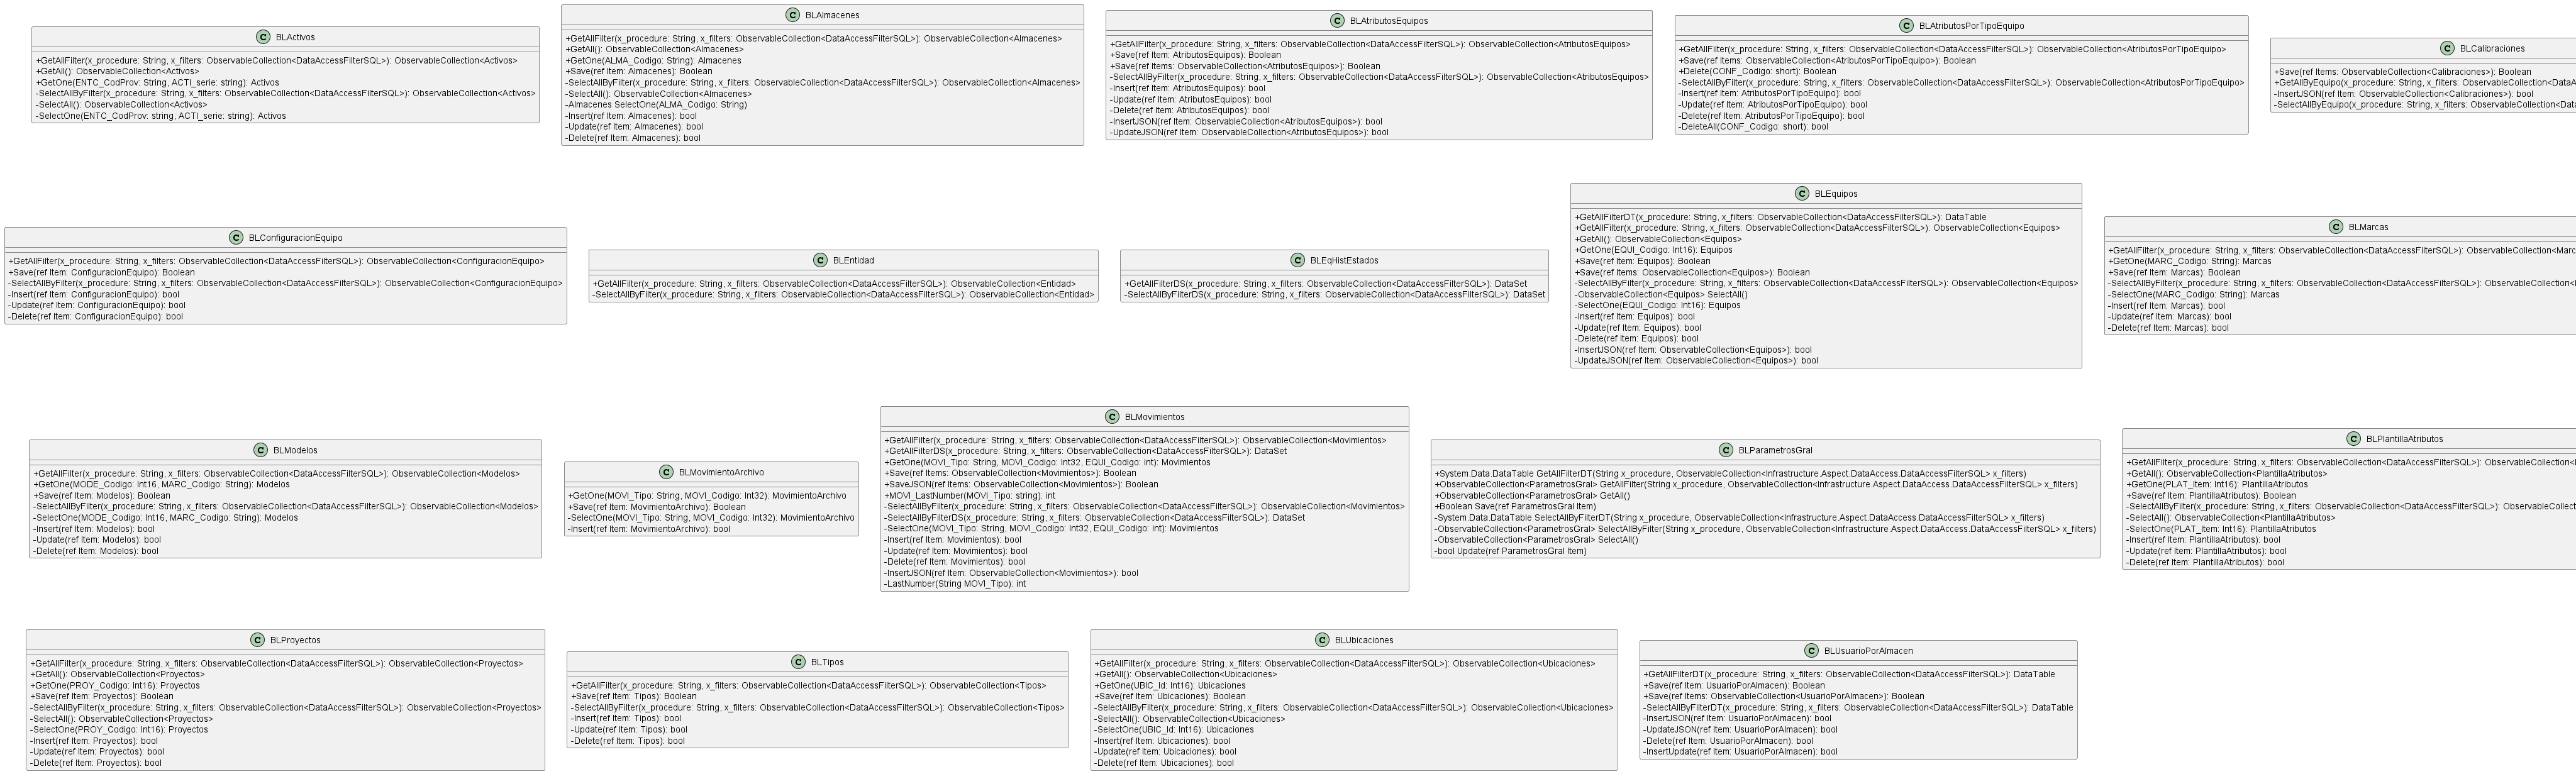
\includegraphics[scale=0.1588, angle=90]{./diagrams/BusinessLogic/BusinessLogic.pdf}
\end{figure}
\end{document}
